\documentclass{standalone}
\usepackage{ tikz }
\usepackage{ xparse }
\input{macros/all}

\begin{document}
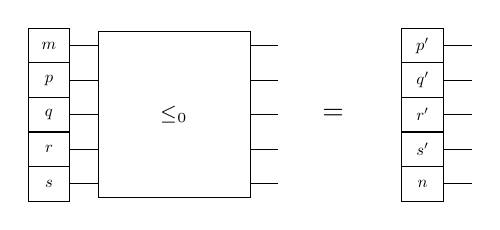
\begin{tikzpicture}[yscale=-1,x=1em,y=1.25em]
        
    \node[draw, minimum height = 1.25em, minimum width = 1.5em, anchor = east] at (0,0){\scalebox{0.6}{$m$}};
    \node[draw, minimum height = 1.25em, minimum width = 1.5em, anchor = east] at (0,1){\scalebox{0.6}{$p$}};
    \node[draw, minimum height = 1.25em, minimum width = 1.5em, anchor = east] at (0,2){\scalebox{0.6}{$q$}};
    \node[draw, minimum height = 1.25em, minimum width = 1.5em, anchor = east] at (0,3){\scalebox{0.6}{$r$}};
    \node[draw, minimum height = 1.25em, minimum width = 1.5em, anchor = east] at (0,4){\scalebox{0.6}{$s$}};

    \draw [rounded corners] (0,0) -- (1,0);
    \draw [rounded corners] (0,1) -- (1,1);
    \draw [rounded corners] (0,2) -- (1,2);
    \draw [rounded corners] (0,3) -- (1,3);
    \draw [rounded corners] (0,4) -- (1,4);

    \node[draw, minimum height = 6em, minimum width = 5.5em, anchor = west] at (1, 2){$\shuffle_{\leq_0}$};

    \draw [rounded corners] (6.5,0) -- (7.5,0);
    \draw [rounded corners] (6.5,1) -- (7.5,1);
    \draw [rounded corners] (6.5,2) -- (7.5,2);
    \draw [rounded corners] (6.5,3) -- (7.5,3);
    \draw [rounded corners] (6.5,4) -- (7.5,4);

    \node at (9.5,2){$=$};

    \node[draw, minimum height = 1.25em, minimum width = 1.5em, anchor = east] at (13.5,0){\scalebox{0.6}{$p'$}};
    \node[draw, minimum height = 1.25em, minimum width = 1.5em, anchor = east] at (13.5,1){\scalebox{0.6}{$q'$}};
    \node[draw, minimum height = 1.25em, minimum width = 1.5em, anchor = east] at (13.5,2){\scalebox{0.6}{$r'$}};
    \node[draw, minimum height = 1.25em, minimum width = 1.5em, anchor = east] at (13.5,3){\scalebox{0.6}{$s'$}};
    \node[draw, minimum height = 1.25em, minimum width = 1.5em, anchor = east] at (13.5,4){\scalebox{0.6}{$n$}};

    \draw [rounded corners] (13.5,0) -- (14.5,0);
    \draw [rounded corners] (13.5,1) -- (14.5,1);
    \draw [rounded corners] (13.5,2) -- (14.5,2);
    \draw [rounded corners] (13.5,3) -- (14.5,3);
    \draw [rounded corners] (13.5,4) -- (14.5,4);

\end{tikzpicture}
\end{document}